\clearpage
\figurepagelayout

\begin{figure}[h]
\caption{Éberség a Légzésre (\emph{Ānāpānasati})}\label{fig-mindfulness-of-breathing}
\bigskip
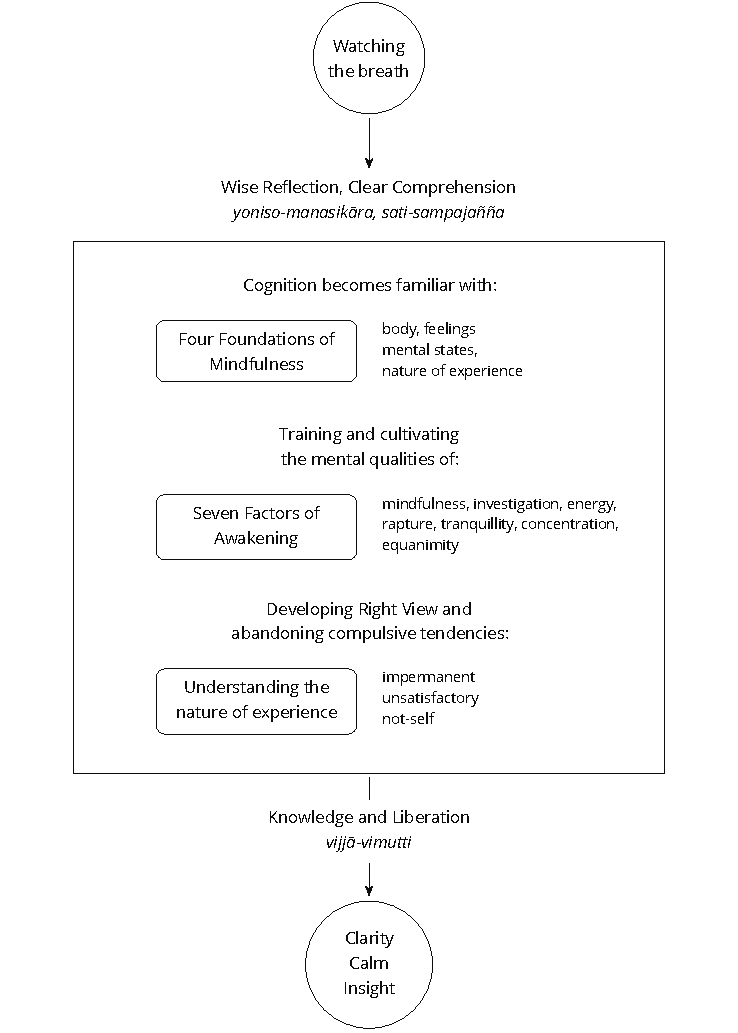
\includegraphics[width=\linewidth]{./manuscript/tex/diagrams/mindfulness-of-breathing.pdf}
\end{figure}

\clearpage
\normalpagelayout

\section{A Lélegzés Tudatosságáról (részlet)}

{\centering
\emph{\href{https://a-buddha-ujja.hu/mn-118/hu/farkas-pal}{MN 118}, Ānāpānasati Sutta}
\par}

{
\setlength{\parindent}{0pt}\setlength{\parskip}{5pt}
\fontsize{9.5}{14}\selectfont

Szerzetesek, a légzés tudatossága, fejlesztve és újra meg újra gyakorolva nagy
eredményt, nagy hasznot hoz, szerzetesek, a légzés tudatossága, fejlesztve és
újra meg újra gyakorolva kiteljesíti a tudatosság négy megalapozását, a
tudatosság négy megalapozása, fejlesztve és újra meg újra gyakorolva kiteljesíti
a megvilágosodás hét tényezőjét, a megvilágosodás hét tényezője, fejlesztve és
újra meg újra gyakorolva kiteljesíti a tisztánlátásból fakadó megszabadulást.

És fejlesztve, szerzetesek, újra meg újra gyakorolva, hogyan hoz a légzés
tudatossága nagy eredményt, nagy hasznot?

E tanítás szerint a szerzetes kimegy az erdőbe, vagy egy fa tövébe, vagy egy
néptelen helyre, keresztbetett lábakkal leül, kiegyenesíti a testét, felkeltvén
tudatosságát (maga előtt).

Tudatosan lélegzik be, tudatosan lélegzik ki.

\textbf{A Test}

Hosszan be- és kilélegezvén tudja,\\ `Hosszan lélegzem be \& ki'.

Röviden be- és kilélegezvén tudja,\\ `Röviden lélegzem be \& ki'.

Így gyakorol:\\ `A teljes testet tapasztalva lélegzem be \& ki'.

Így gyakorol:\\ `A testi képző erőket elnyugtatva, lélegzem be \& ki'.

\clearpage

\textbf{Az Érzések}

Így gyakorol:

`Örömöt tapasztalva lélegzem be \& ki'.

`Boldogságot tapasztalva lélegzem be \& ki'.

`A tudati képző erőket tapasztalva lélegzem be \& ki'.

`A tudati képző erőket elnyugtatva lélegzem be \& ki'.

\textbf{A Tudat}

Így gyakorol:

`A tudatot tapasztalva lélegzem be \& ki'.

`A tudatot felvidítva lélegzem be \& ki'.

`A tudatot összpontosítva lélegzem be \& ki'.

`A tudatot megszabadítva lélegzem be \& ki'.

\textbf{A Tudat Tartalma}

Így gyakorol:

`A mulandóság fölött szemlélődve lélegzem be \& ki'.

`Az elenyészés fölött szemlélődve lélegzem be \& ki'.

`A megszűnés fölött szemlélődve lélegzem be \& ki'.

`Az eloldódás fölött szemlélődve lélegzem be \& ki'.

\bigskip

Ily módon hoz a légzés tudatossága, fejlesztve és újra meg újra gyakorolva, nagy eredményt, nagy hasznot.

}
